\section {Updated predictions of numbers of single $\mu$-like ring events in SuperK}
\label{sec:updated_predictions}

In this section we present plots and tables comparing the GENIE and NEUT predictions (after extrapolation) of the numbers of 1 $\mu$-like ring events in SuperK under various oscillation hypotheses.

In Figs.\ \ref{fig:genie_mode_contrib_noosc} and \ref{fig:neut_mode_contrib_noosc} are shown,
respectively, the GENIE and NEUT predicted (after extrapolation)
non-oscillated reconstructed-energy spectrum of 1 $\mu$-like ring events 
passing the so-called `tight' cuts (see Tab.\ 1 of Ref.\ \cite{OurRun1DisappAnalysis}). 
The contributions from various true neutrino reaction modes are also shown. 
Figs.\ \ref{fig:genie_mode_contrib_noosc_logy} and \ref{fig:neut_mode_contrib_noosc_logy} show
the same distribution with a log scale so that the contribution from all
non-$\nu_{\mu}$ CCQE backgrounds can be seen.
The corresponding predictions for oscillations with typical parameters
($sin^{2}2\theta_{23}$=1.0 and $|\Delta m^{2}_{23}|$=2.32$\times10^{-3}$ $eV^{2}/c^{4}$)
are shown in 
Figs.\ \ref{fig:genie_mode_contrib_2p32Em3_1p0} and \ref{fig:genie_mode_contrib_2p32Em3_1p0_logy} for GENIE and 
Figs.\ \ref{fig:neut_mode_contrib_2p32Em3_1p0} and \ref{fig:neut_mode_contrib_2p32Em3_1p0_logy} for NEUT.

A summary is given in Tab.\ \ref{tab:genie_neut_mode_contrib} for both oscillated and
non-oscillated scenarios  of
the expected numbers of events (after extrapolation) in SuperK and the
nominal expected contributions from various true neutrino reaction
modes (corresponding to the different SuperK MC templates used in this
analysis, see Sec. 2.4 of Ref. \cite{OurRun1DisappAnalysis}).

In Fig.\ \ref{fig:genie_nsk_osc_param_grid} we show the GENIE prediction of the integrated number 
of 1 $\mu$-like ring events (after extrapolation) for 
an extended grid of $sin^{2}2\theta_{23}$ and $\Delta m^{2}_{23}$ values.
The corresponding plot for NEUT is shown in Fig.\ \ref{fig:neut_nsk_osc_param_grid}.
The same plots are shown in Fig.\ \ref{fig:genie_nsk_osc_param_grid_zoom}
(GENIE) and Fig.\ \ref{fig:neut_nsk_osc_param_grid_zoom} (NEUT)
but zoomed in around the MINOS 2011 best-fit values.

The estimated uncertainty in the number of 1 $\mu$-like ring SuperK events (after extrapolation) due to all the sources of uncertainty listed in
Tab.\ \ref{tab:input_uncertainties}
is shown in for both GENIE and NEUT in
Tab.\ \ref{table:dnsk_noosc} (no oscillation) and
Tab.\ \ref{table:dnsk_minos11} (oscillations with 
$sin^{2}2\theta_{23}$ = 1.0 and $|\Delta m^{2}_{23}|$ = 2.32$\times10^{-3}$ $eV^{2}/c^{4}$).
The error envelope of the 1 $\mu$-like ring event reconstructed-energy spectrum (after extrapolation)
for the latter typical oscillation hypothesis is shown 
in Fig.\ \ref{fig:genie-sk-err-envelope-minos11} for GENIE and
in Fig.\ \ref{fig:neut-sk-err-envelope-minos11} for NEUT.

%
% Number of events GENIE & NEUT
%

\begin{table}
\centering
\begin{tabular}{| c || c | c || c | c | }
\hline
   & \multicolumn{2}{c||} { (a) }
   & \multicolumn{2}{c| } { (b) }\\
                                         & GENIE              & NEUT                & GENIE               & NEUT  \\
\hline
\hline
Total                                    & 101.717            & 103.593             &  28.394             &   29.177              \\
$\nu_{\mu}$ CCQE                         &  82.074 (80.688\%) &  82.348 (79.491\%)  &  16.520 (58.182\%)  &   16.731 (57.343\%)   \\
$\nu_{\mu}$ CC1$\pi$                     &  12.895 (12.677\%) &  13.986 (13.501\%)  &   6.676 (23.510\%)  &    7.014 (24.040\%)   \\
$\nu_{\mu}$ CCother                      &   1.315  (1.292\%) &   2.306  (2.226\%)  &   1.107  (3.900\%)  &    1.800  (6.168\%)   \\
$\nu_{\mu}$($\nu_{\tau}$) NC             &   2.116  (2.080\%) &   1.682  (1.624\%)  &   2.116  (7.452\%)  &    1.682  (5.766\%)   \\
$\bar{\nu_{\mu}}$ CCQE                   &   2.111  (2.076\%) &   2.186  (2.110\%)  &   1.045  (3.679\%)  &    1.112  (3.813\%)   \\
$\bar{\nu_{\mu}}$ CC1$\pi$               &   0.885  (0.870\%) &   0.698  (0.674\%)  &   0.634  (2.231\%)  &    0.510  (1.748\%)   \\
$\bar{\nu_{\mu}}$ CCother                &   0.131  (0.129\%) &   0.227  (0.219\%)  &   0.106  (0.371\%)  &    0.167  (0.572\%)   \\
$\bar{\nu_{\mu}}$($\bar{\nu_{\tau}}$) NC &   0.117  (0.114\%) &   0.093  (0.090\%)  &   0.117  (0.411\%)  &    0.093  (0.319\%)   \\
$\nu_{e}$ CCQE                           &   0.007  (0.007\%) &   0.008  (0.007\%)  &   0.007  (0.025\%)  &    0.008  (0.026\%)   \\
$\nu_{e}$ CC1$\pi$                       &   0.004  (0.004\%) &   0.005  (0.005\%)  &   0.004  (0.015\%)  &    0.005  (0.016\%)   \\
$\nu_{e}$ CCother                        &   0.001  (0.001\%) &   0.002  (0.002\%)  &   0.001  (0.004\%)  &    0.002  (0.006\%)   \\
$\nu_{e}$ NC                             &   0.062  (0.061\%) &   0.054  (0.052\%)  &   0.062  (0.220\%)  &    0.054  (0.184\%)   \\
\hline
\end{tabular}
\caption{ 
  Expected numbers of SuperK 1 $\mu$-like ring events from GENIE and NEUT (after extrapolation) for
  (a) no oscillation and
  (b) oscillations with $sin^{2}2\theta_{23}$ = 1.0 and $|\Delta m^{2}_{23}|$ = 2.32$\times10^{-3}$ $eV^{2}/c^{4}$.
}
\label{tab:genie_neut_mode_contrib}
\end{table}

%
% GENIE and NEUT 1-ring Ereco spectrum: No oscillations
%

\begin{figure}[ht]
\begin{minipage}[t]{0.48\linewidth}
\centering
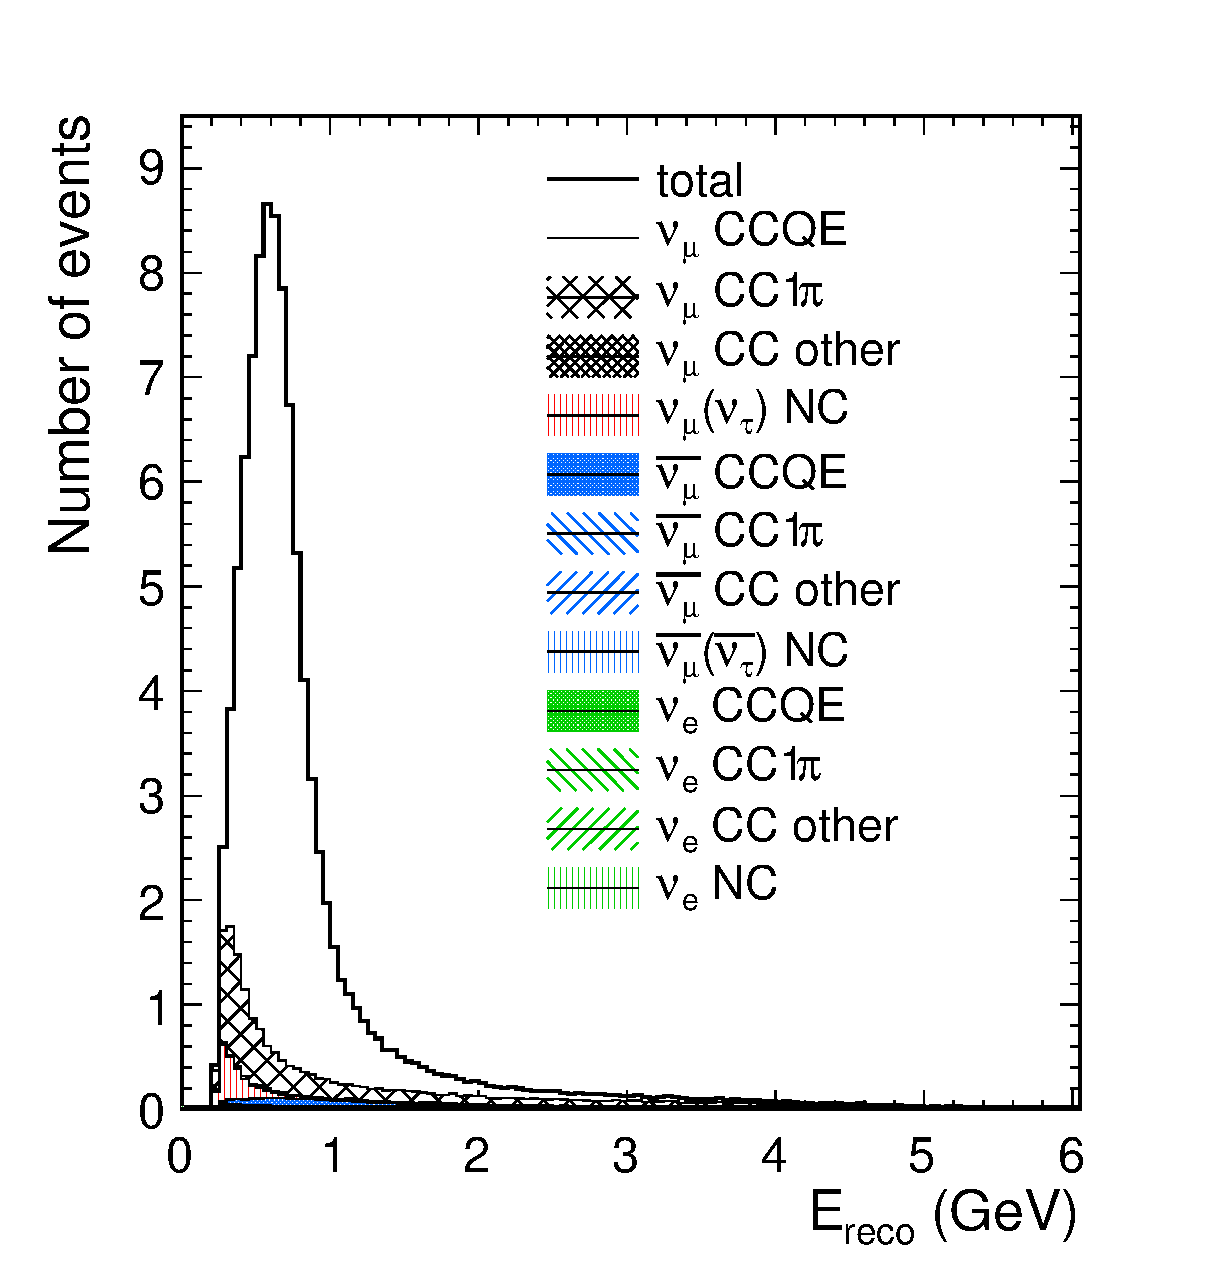
\includegraphics[width=19pc,height=19pc]{./images/predicted_spectrum/nominal/genie_contrib_noosc.eps}
\caption{
  Predicted non-oscillated reconstructed-energy spectrum of 1 $\mu$-like ring events (after extrapolation)
  and contributions from various true neutrino reaction modes (GENIE)
}
\label{fig:genie_mode_contrib_noosc}
\end{minipage}
\hspace{0.04\linewidth}
\begin{minipage}[t]{0.48\linewidth}
\centering
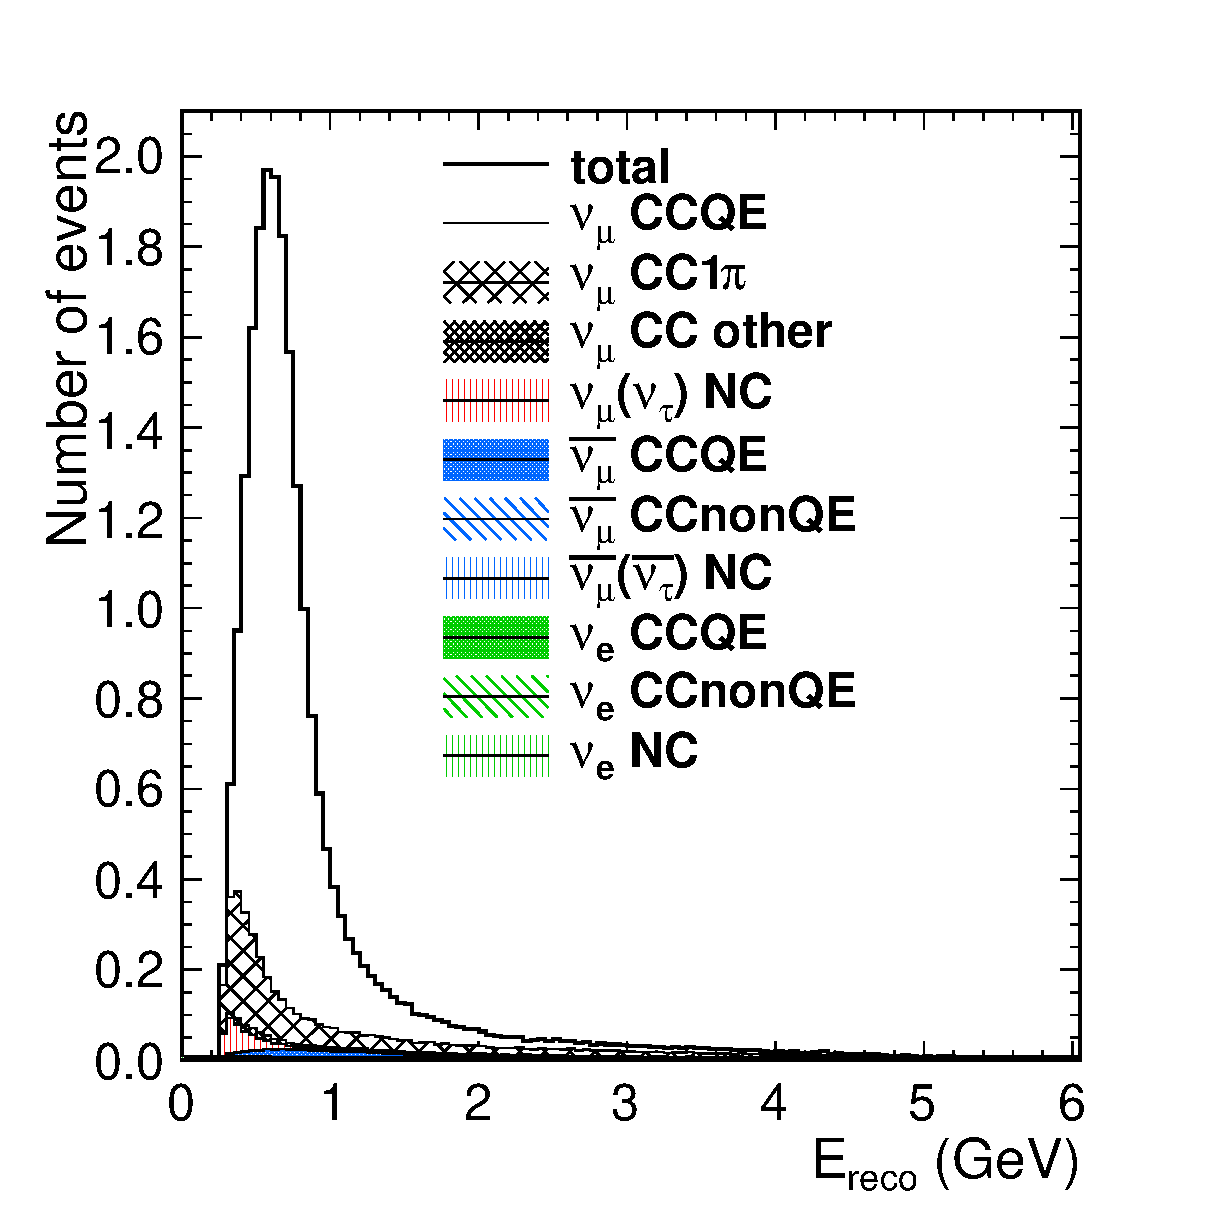
\includegraphics[width=19.5pc,height=19pc]{images/predicted_spectrum/nominal/neut_contrib_noosc.eps}
\caption{
  Predicted non-oscillated reconstructed-energy spectrum of 1 $\mu$-like ring events (after extrapolation)
  and contributions from various true neutrino reaction modes (NEUT)
}
\label{fig:neut_mode_contrib_noosc}
\end{minipage}
\end{figure}


% as above but in log-scale

\begin{figure}[ht]
\begin{minipage}[t]{0.48\linewidth}
\centering
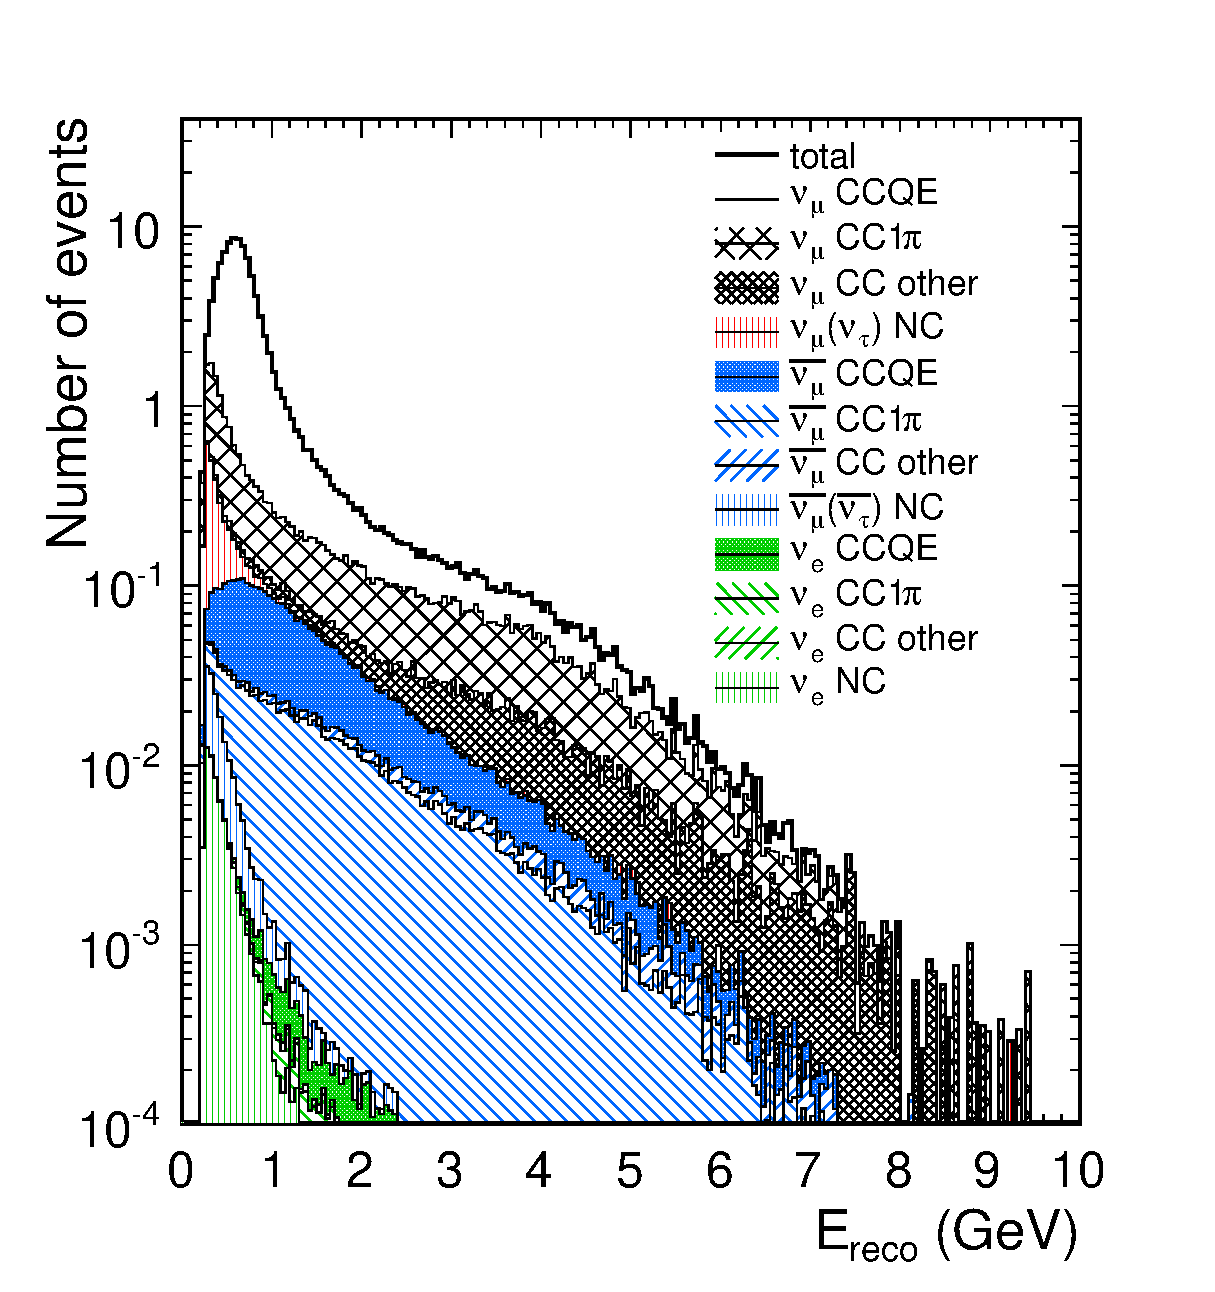
\includegraphics[width=19pc,height=19pc]{./images/predicted_spectrum/nominal/genie_contrib_noosc_logy.eps}
\caption{
  Predicted non-oscillated reconstructed-energy spectrum of 1 $\mu$-like ring events (after extrapolation)
  and contributions from various true neutrino reaction modes (GENIE)
}
\label{fig:genie_mode_contrib_noosc_logy}
\end{minipage}
\hspace{0.04\linewidth}
\begin{minipage}[t]{0.48\linewidth}
\centering
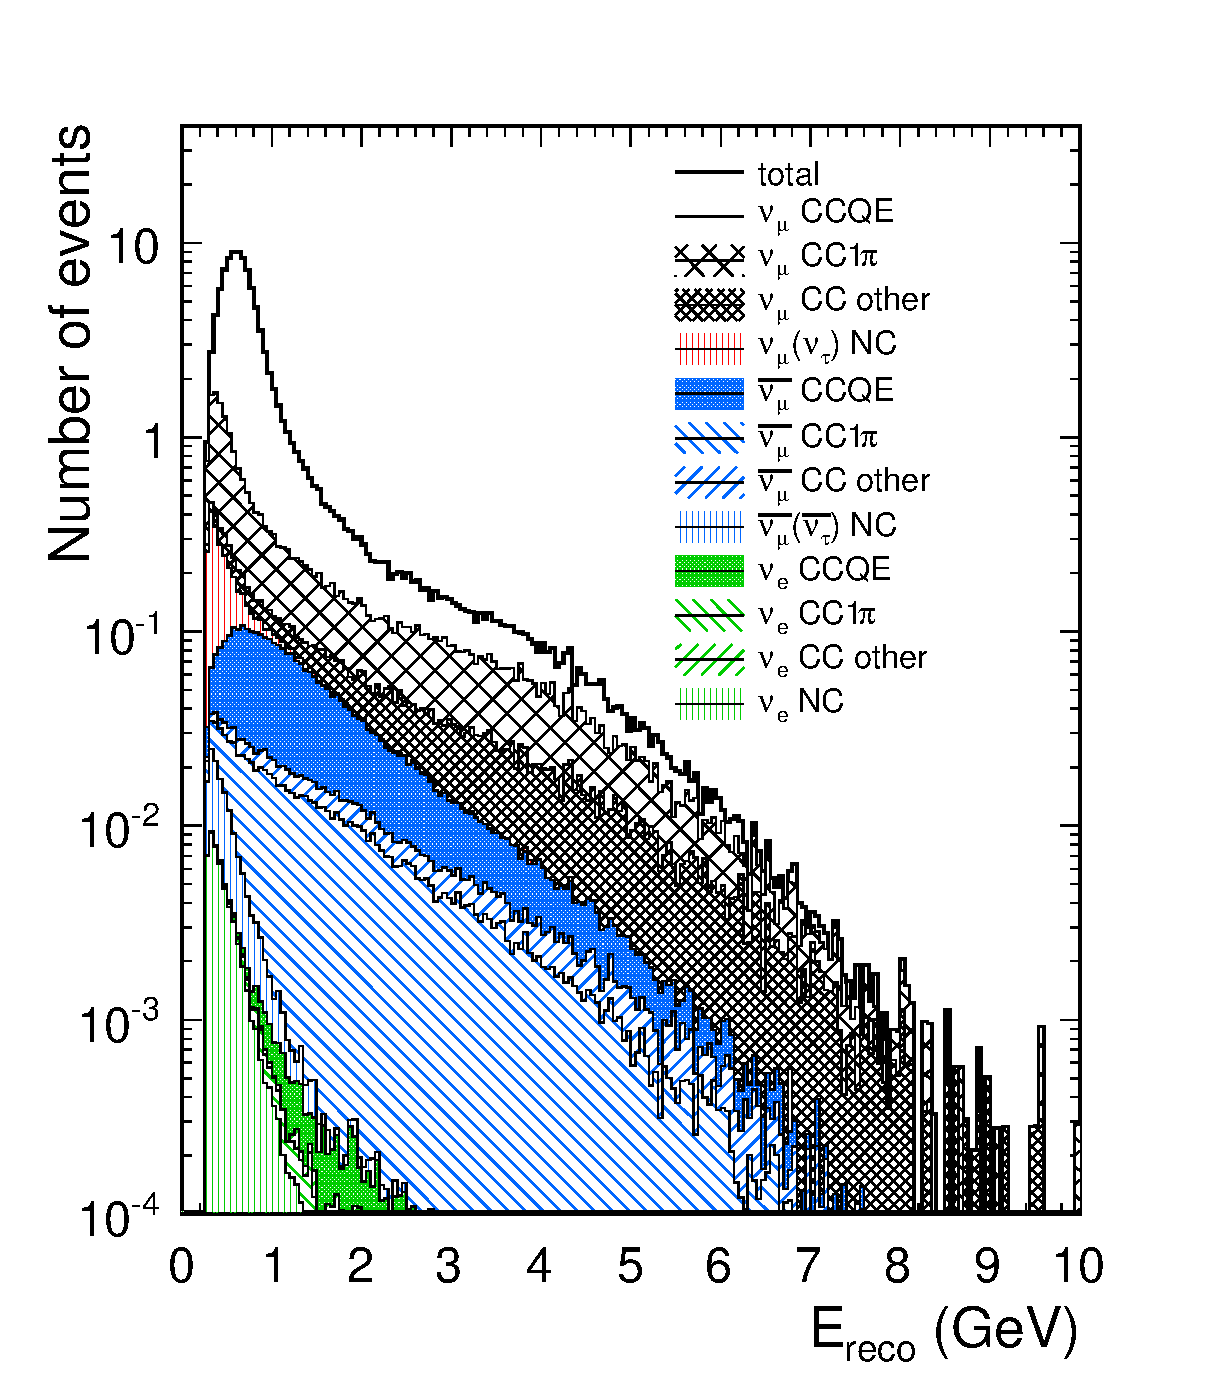
\includegraphics[width=19.5pc,height=19pc]{images/predicted_spectrum/nominal/neut_contrib_noosc_logy.eps}
\caption{
  Predicted non-oscillated reconstructed-energy spectrum of 1 $\mu$-like ring events (after extrapolation)
  and contributions from various true neutrino reaction modes (NEUT)
}
\label{fig:neut_mode_contrib_noosc_logy}
\end{minipage}
\end{figure}


%
% GENIE and NEUT 1-ring Ereco spectrum: MINOS-2011 oscillation params
%

\begin{figure}[ht]
\begin{minipage}[t]{0.48\linewidth}
\centering
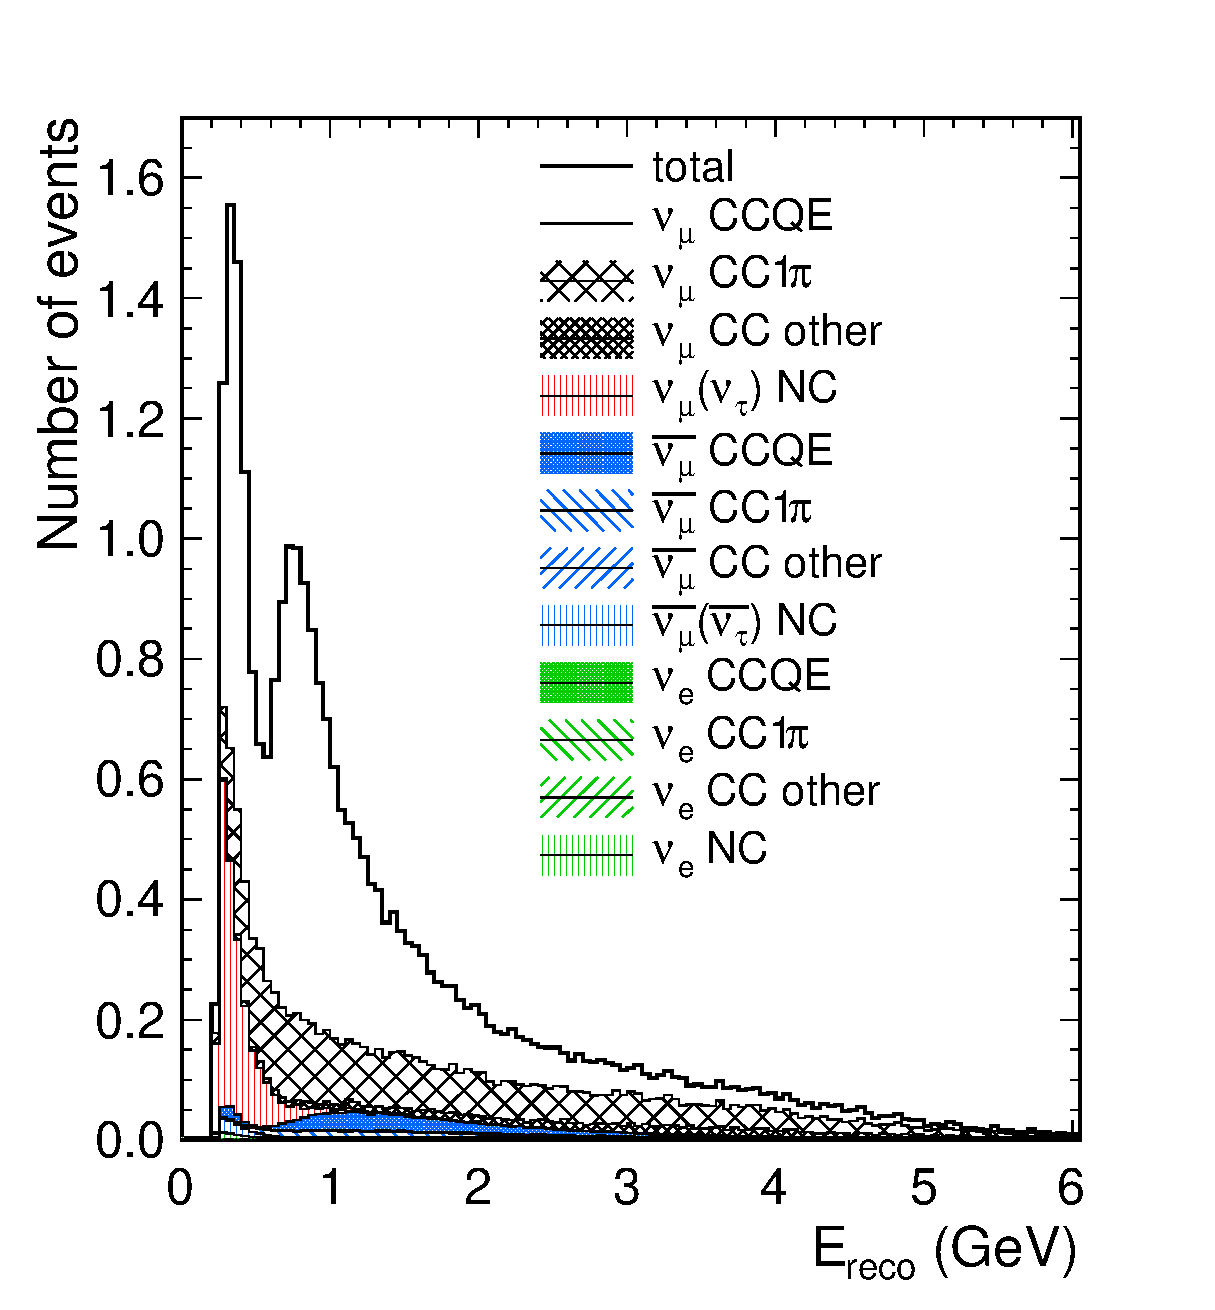
\includegraphics[width=19pc,height=19pc]{./images/predicted_spectrum/nominal/genie_contrib_2p32Em3_1p0.eps}
\caption{
  Predicted oscillated ($sin^{2}2\theta_{23}$ = 1.0 and $|\Delta m^{2}_{23}|$ = 2.32$\times10^{-3}$ $eV^{2}/c^{4}$)
  reconstructed-energy spectrum of 1 $\mu$-like ring events (after extrapolation)
  and contributions from various true neutrino reaction modes (GENIE)
}
\label{fig:genie_mode_contrib_2p32Em3_1p0}
\end{minipage}
\hspace{0.04\linewidth}
\begin{minipage}[t]{0.48\linewidth}
\centering
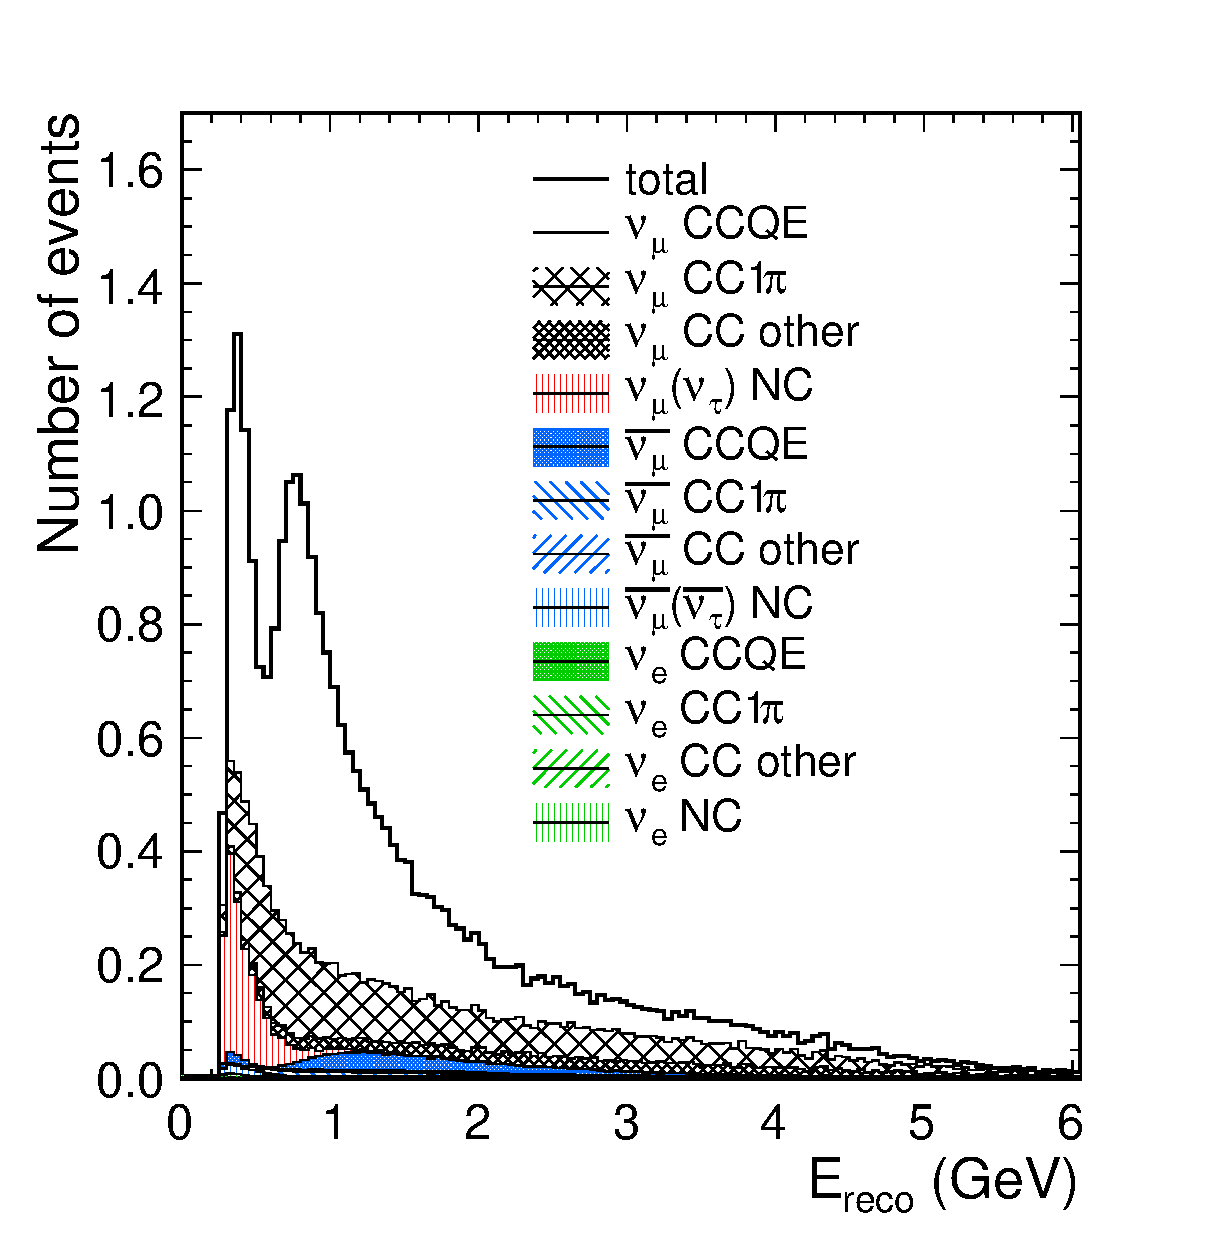
\includegraphics[width=19pc,height=19pc]{images/predicted_spectrum/nominal/neut_contrib_2p32Em3_1p0.eps}
\caption{
  Predicted oscillated ($sin^{2}2\theta_{23}$ = 1.0 and $|\Delta m^{2}_{23}|$ = 2.32$\times10^{-3}$ $eV^{2}/c^{4}$)
  reconstructed-energy spectrum of 1 $\mu$-like ring events (after extrapolation)
  and contributions from various true neutrino reaction modes (NEUT)
}
\label{fig:neut_mode_contrib_2p32Em3_1p0}
\end{minipage}
\end{figure}


% as above but in log-scale

\begin{figure}[ht]
\begin{minipage}[t]{0.48\linewidth}
\centering
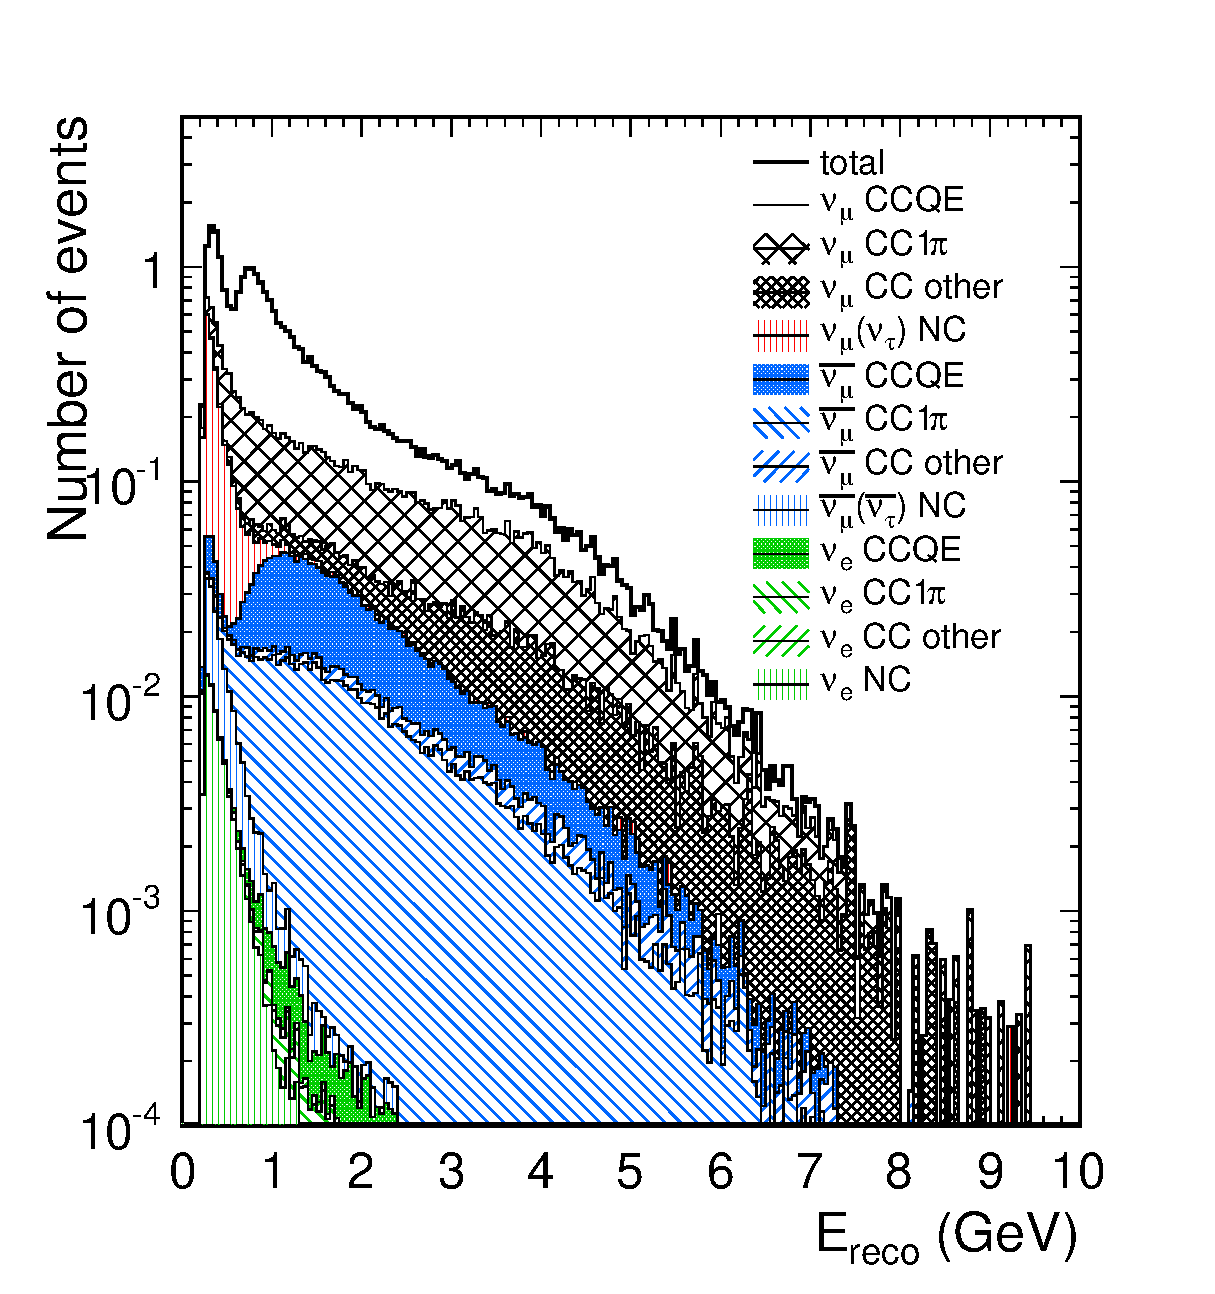
\includegraphics[width=19pc,height=19pc]{./images/predicted_spectrum/nominal/genie_contrib_2p32Em3_1p0_logy.eps}
\caption{
  Predicted oscillated ($sin^{2}2\theta_{23}$ = 1.0 and $|\Delta m^{2}_{23}|$ = 2.32$\times10^{-3}$ $eV^{2}/c^{4}$)
  reconstructed-energy spectrum of 1 $\mu$-like ring events (after extrapolation)
  and contributions from various true neutrino reaction modes (GENIE)
}
\label{fig:genie_mode_contrib_2p32Em3_1p0_logy}
\end{minipage}
\hspace{0.04\linewidth}
\begin{minipage}[t]{0.48\linewidth}
\centering
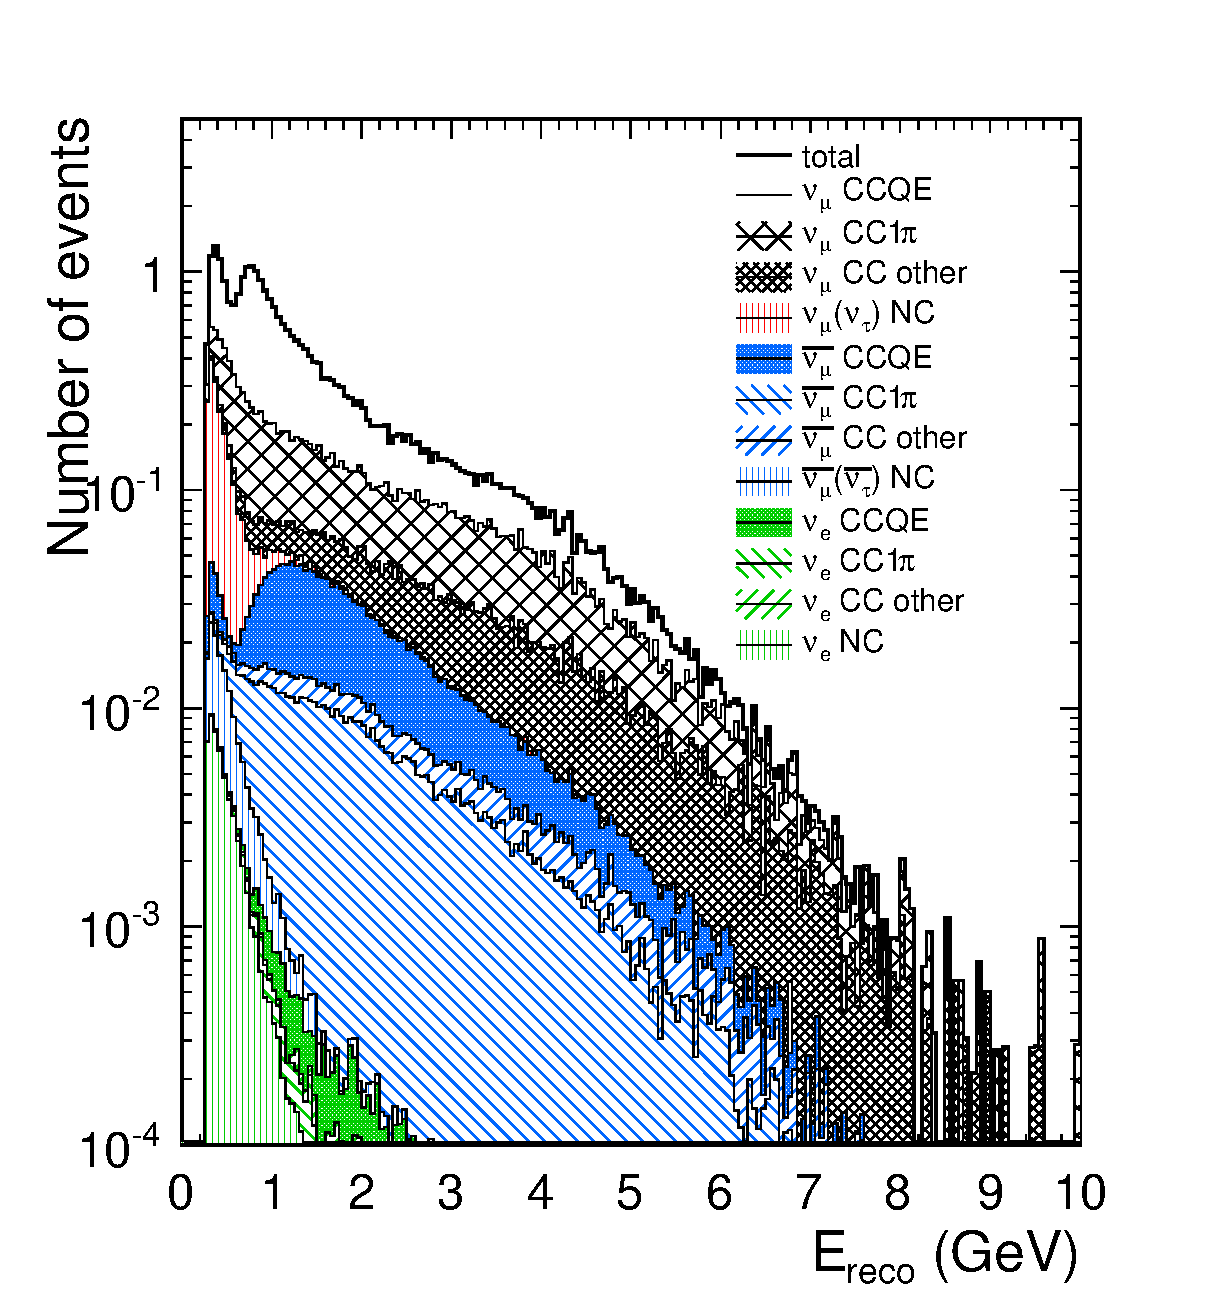
\includegraphics[width=19pc,height=19pc]{images/predicted_spectrum/nominal/neut_contrib_2p32Em3_1p0_logy.eps}
\caption{
  Predicted oscillated ($sin^{2}2\theta_{23}$ = 1.0 and $|\Delta m^{2}_{23}|$ = 2.32$\times10^{-3}$ $eV^{2}/c^{4}$)
  reconstructed-energy spectrum of 1 $\mu$-like ring events (after extrapolation)
  and contributions from various true neutrino reaction modes (NEUT)
}
\label{fig:neut_mode_contrib_2p32Em3_1p0_logy}
\end{minipage}
\end{figure}

%
% Nsk vs oscillation parameters
%

\begin{figure}[ht]
\begin{minipage}[t]{0.47\linewidth}
\centering
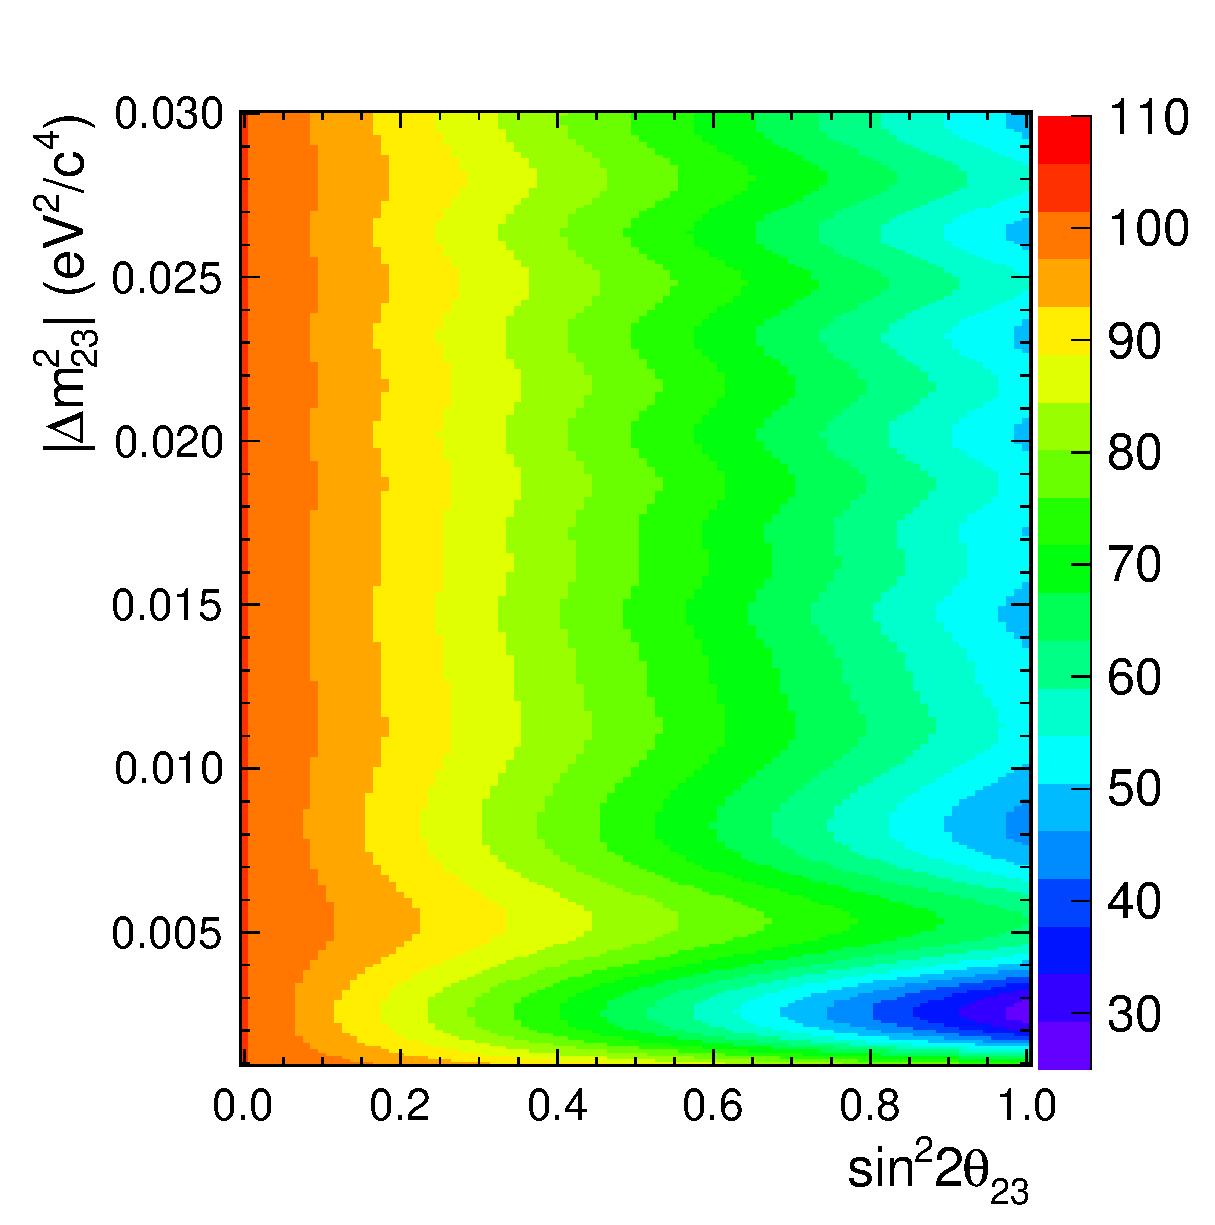
\includegraphics[width=18pc,height=19pc]{./images/predicted_spectrum/nominal/genie_nsk_osc.eps}
\caption{
  Expected number of 1 $\mu$-like ring events (after extrapolation) in the 0-10 GeV reconstructed
  energy range (GENIE)
}
\label{fig:genie_nsk_osc_param_grid}
\end{minipage}
\hspace{0.06\linewidth}
\begin{minipage}[t]{0.47\linewidth}
\centering
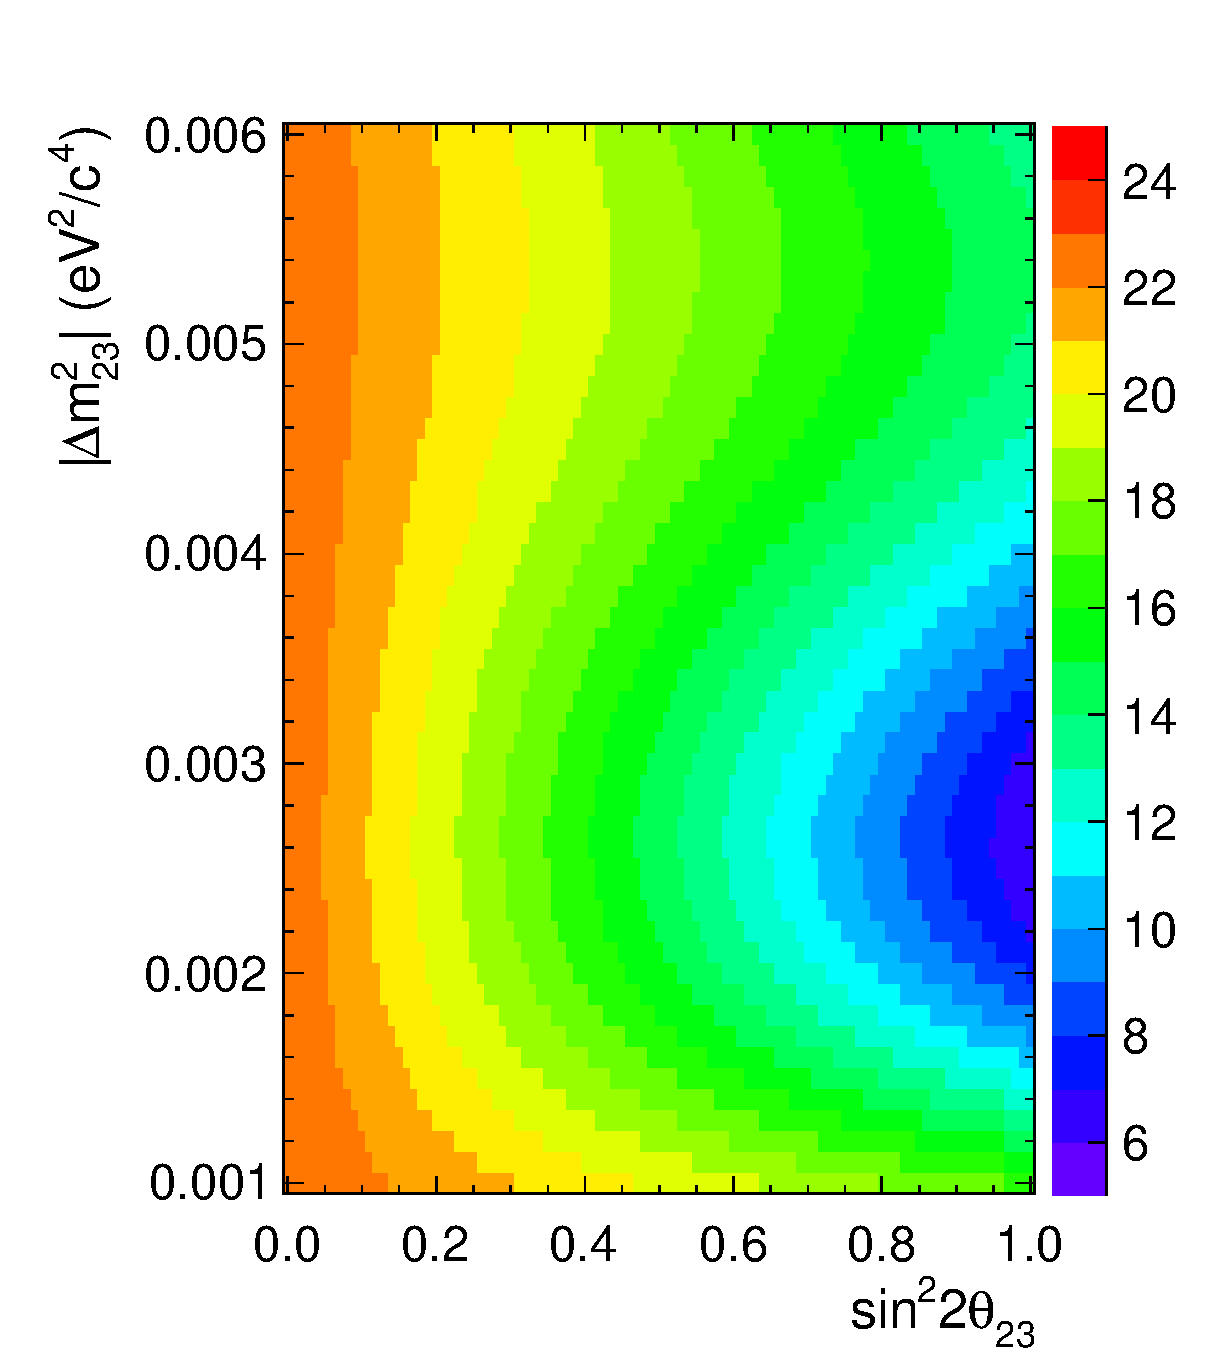
\includegraphics[width=18pc,height=19pc]{images/predicted_spectrum/nominal/neut_nsk_osc.eps}
\caption{
  Expected number of 1 $\mu$-like ring events (after extrapolation) in the 0-10 GeV reconstructed
  energy range (NEUT)
}
\label{fig:neut_nsk_osc_param_grid}
\end{minipage}
\end{figure}


%
% Nsk vs oscillation parameters
%

\begin{figure}[ht]
\begin{minipage}[t]{0.47\linewidth}
\centering
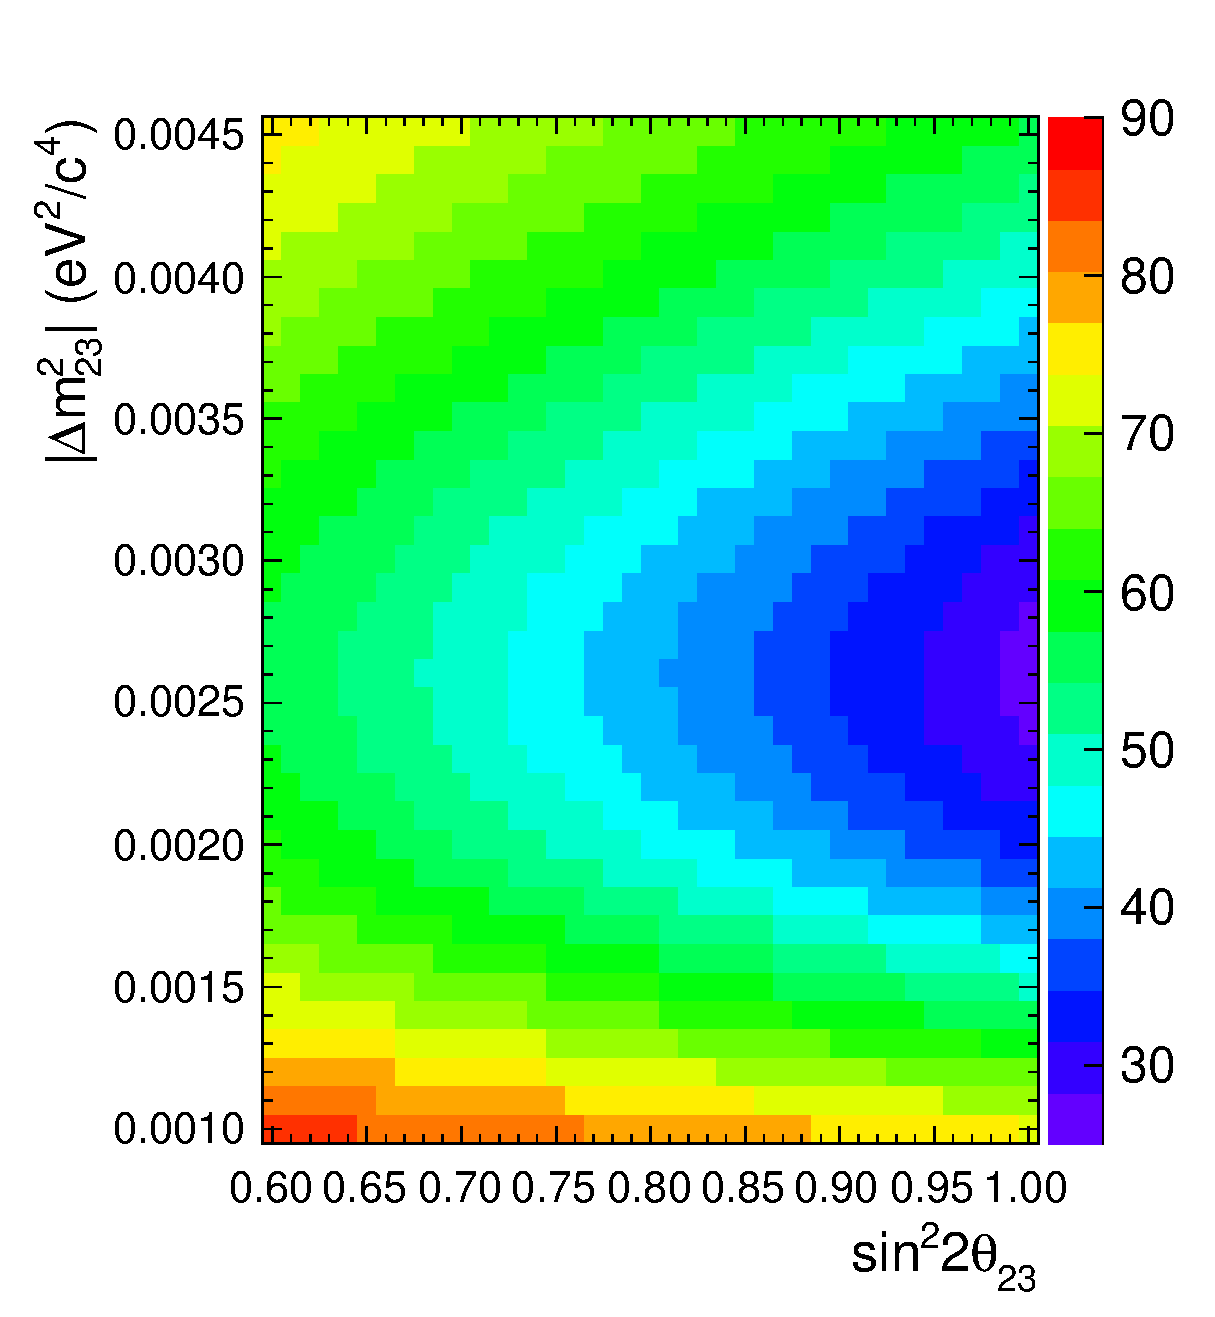
\includegraphics[width=18pc,height=19pc]{./images/predicted_spectrum/nominal/genie_nsk_osc_zoom.eps}
\caption{
  Expected number of 1 $\mu$-like ring events (after extrapolation) in the 0-10 GeV reconstructed
  energy range, zoomed around the MINOS 2011 best-fit values (GENIE)
}
\label{fig:genie_nsk_osc_param_grid_zoom}
\end{minipage}
\hspace{0.06\linewidth}
\begin{minipage}[t]{0.47\linewidth}
\centering
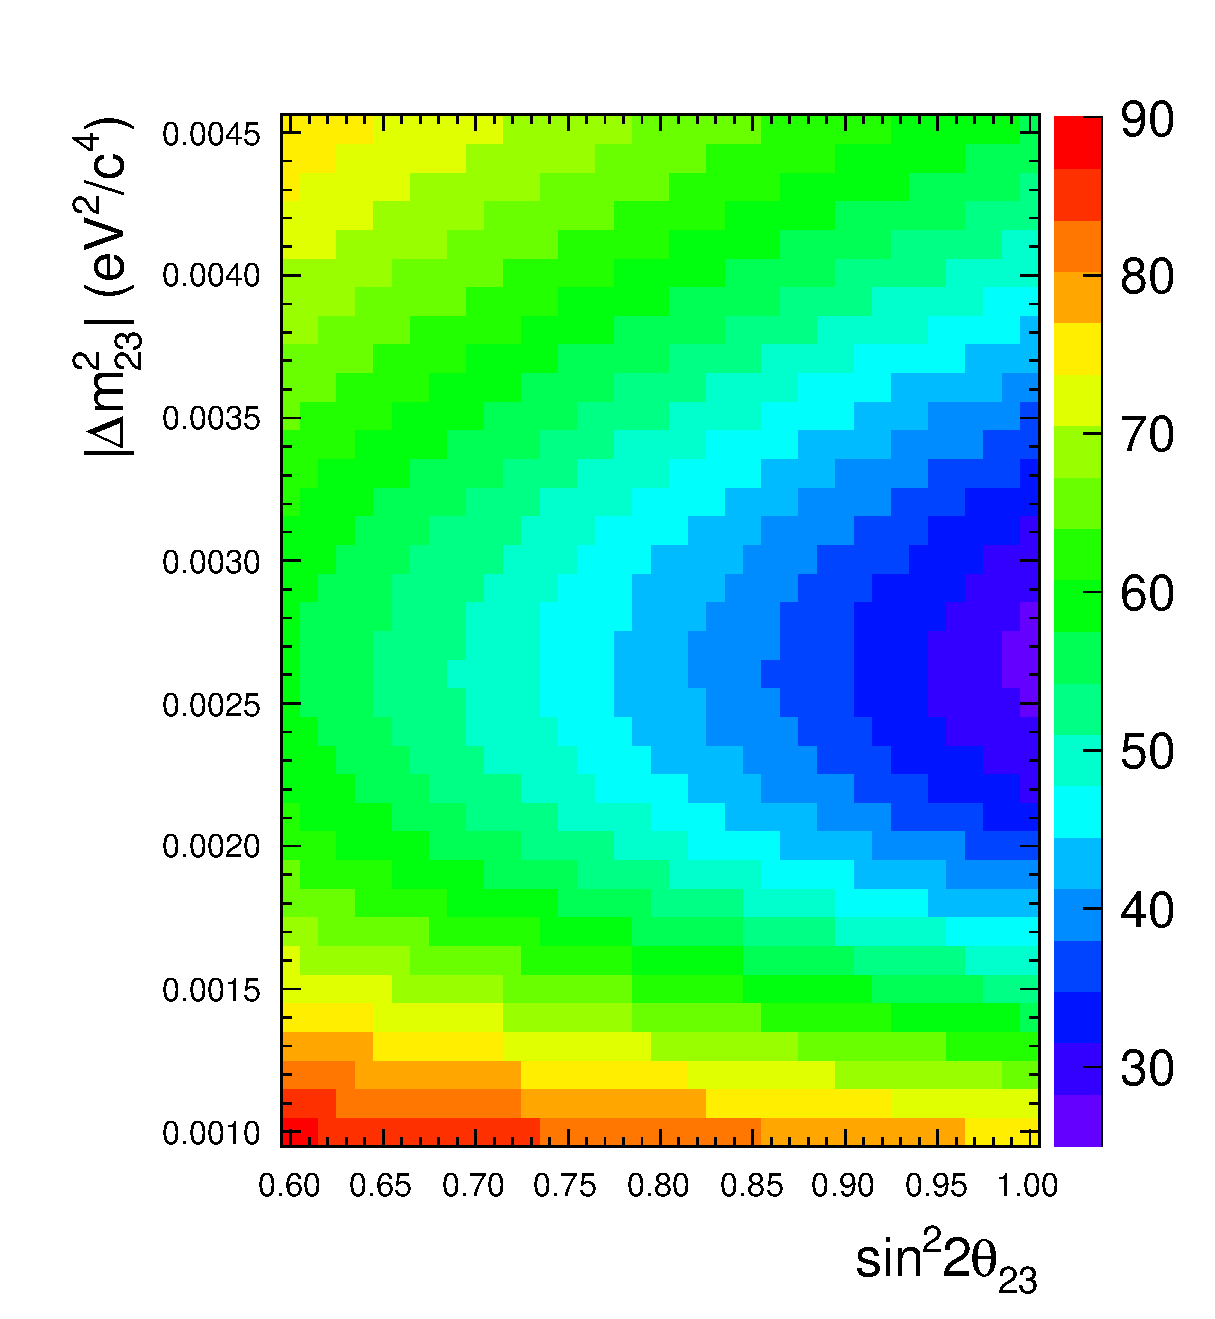
\includegraphics[width=18pc,height=19pc]{images/predicted_spectrum/nominal/neut_nsk_osc_zoom.eps}
\caption{
  Expected number of 1 $\mu$-like ring events (after extrapolation) in the 0-10 GeV reconstructed
  energy range, zoomed around the MINOS 2011 best-fit values (NEUT)
}
\label{fig:neut_nsk_osc_param_grid_zoom}
\end{minipage}
\end{figure}

\begin{table*}[htb]
\center
\renewcommand{\arraystretch}{1.75} % enlarge line spacing
\begin{tabular}{|c|c|c|}
\hline
       & GENIE & NEUT \\
Error source  &
  $\delta{N^{exp}_{SK}}/N^{exp}_{SK}$  &
  $\delta{N^{exp}_{SK}}/N^{exp}_{SK}$  \\
\hline
SuperK CCQE efficiency (ring-counting)  &   $\pm$2.99\%       &   $\pm$3.06\%       \\
SuperK CCQE efficiency (other)          &   $\pm$1.41\%       &   $\pm$1.39\%       \\
SuperK CCnonQE efficiency               &   $\pm$2.99\%       &   $\pm$3.32\%       \\
SuperK NC efficiency                    &   $\pm$2.51\%       &   $\pm$1.96\%       \\
SuperK $\nu_{e}$ CC efficiency          &   $\pm$0.01\%       &   $\pm$0.01\%       \\
ND280 efficiency                        &   +5.49\% -5.30\%   &   +5.49\% -5.30\%   \\
ND280 normalization                     &   $\pm$2.63\%       &   $\pm$2.62\%       \\
Flux normalization                      &   $\pm$7.29\%       &   $\pm$7.33\%       \\
CCQE cross section                      &   $\pm$4.28\%       &   $\pm$4.05\%       \\
CC1pi/CCQE cross section ratio          &   +2.66\% -2.35\%   &   +2.18\% -1.93\%   \\
CCother/CCQE cross section ratio        &   +5.80\% -5.16\%   &   +5.27\% -4.71\%   \\ 
NC/CCQE cross section ratio             &   +0.68\% -0.66\%   &   +0.81\% -0.78\%   \\
FSI                                     &   $\pm$3.23\%       &   $\pm$3.22\%       \\
\hline
Total                                   &   +13.65\% -13.26\% &   +13.30\% -12.97\% \\
\hline
\end{tabular}\\[2pt]
\caption{
  Effect of 1$\sigma$ systematic parameter variation on the non-oscillated number of 1 $\mu$-like ring events
  predicted by GENIE and NEUT (after extrapolation)
}
\label{table:dnsk_noosc}
\end{table*}



\begin{table*}[htb]
\center
\renewcommand{\arraystretch}{1.75} % enlarge line spacing
\begin{tabular}{|c|c|c|}
\hline
       & GENIE & NEUT \\
Error source  &
  $\delta{N^{exp}_{SK}}/N^{exp}_{SK}$  &
  $\delta{N^{exp}_{SK}}/N^{exp}_{SK}$  \\
\hline
SuperK CCQE efficiency (ring-counting)  &   $\pm$3.04\%       &   $\pm$3.23\%       \\
SuperK CCQE efficiency (other)          &   $\pm$1.05\%       &   $\pm$1.04\%       \\
SuperK CCnonQE efficiency               &   $\pm$6.00\%       &   $\pm$6.51\%       \\
SuperK NC efficiency                    &   $\pm$8.97\%       &   $\pm$6.96\%       \\
SuperK $\nu_{e}$ CC efficiency          &   $\pm$0.04\%       &   $\pm$0.05\%       \\
ND280 efficiency                        &   +5.49\% -5.30\%   &   +5.59\% -5.30\%   \\
ND280 normalization                     &   $\pm$2.63\%       &   $\pm$2.62\%       \\
Flux normalization                      &   $\pm$4.78\%       &   $\pm$4.73\%       \\
CCQE cross section                      &   $\pm$2.78\%       &   $\pm$2.36\%       \\
CC1pi/CCQE cross section ratio          &   +0.22\% -0.25\%   &   +0.52\% -0.59\%   \\
CCother/CCQE cross section ratio        &   +5.04\% -4.48\%   &   +4.10\% -3.67\%   \\ 
NC/CCQE cross section ratio             &   +1.40\% -1.44\%   &   +0.82\% -0.84\%   \\
FSI                                     &   $\pm$5.68\%       &   $\pm$5.80\%       \\
\hline
Total                                   &   +15.94\% -15.72\% &   +14.79\% -14.61\% \\
\hline
\end{tabular}\\[2pt]
\caption{
  Effect of 1$\sigma$ systematic parameter variation on the number of 1 $\mu$-like ring events
  predicted by GENIE and NEUT (after extarpolation)
  assuming oscillations with typical (MINOS 2011) parameters
  ($sin^{2}2\theta_{23}$ = 1.0 and $|\Delta m^{2}_{23}|$ = 2.32$\times10^{-3}$ $eV^{2}/c^{4}$).
}
\label{table:dnsk_minos11}
\end{table*}


%
% GENIE and NEUT 1-ring Ereco spectrum error envelope
%

\begin{figure}[ht]
\begin{minipage}[t]{0.48\linewidth}
\centering
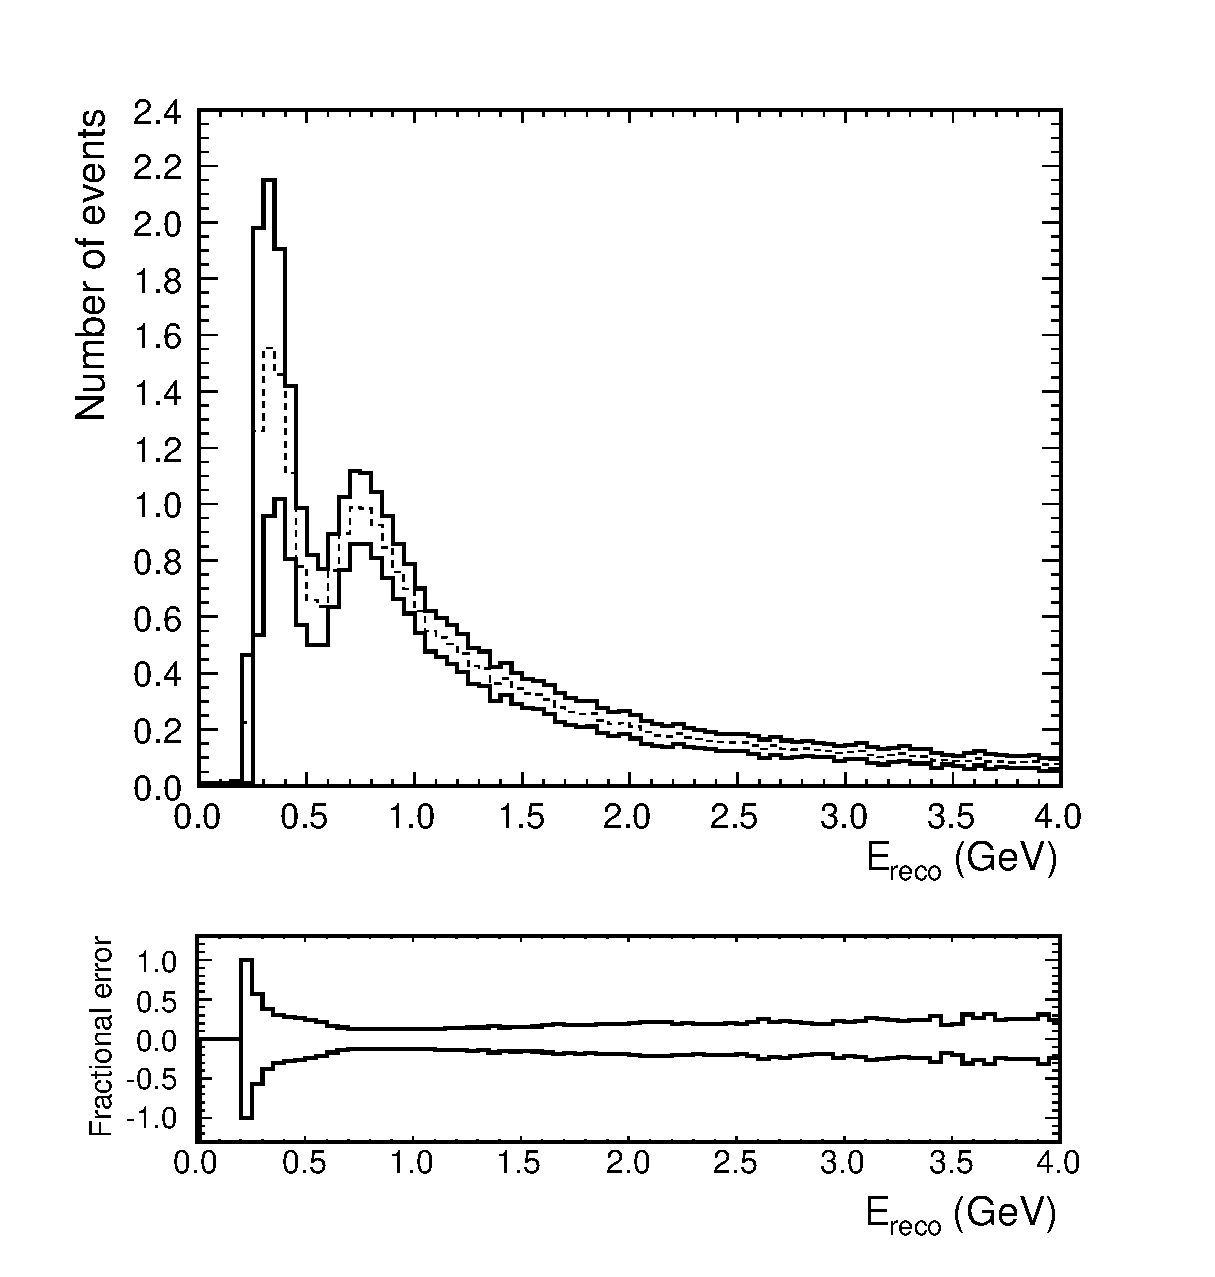
\includegraphics[width=18pc,height=20pc]{./images/predicted_spectrum/systematic_variations/genie-sk-err-envelope-minos11.eps}
\caption{
  Error envelope of 1 $\mu$-like ring event reconstructed-energy spectrum (after extrapolation)
  for oscillations with $sin^{2}2\theta_{23}$ = 1.0 and $|\Delta m^{2}_{23}|$ = 2.32$\times10^{-3}$ $eV^{2}/c^{4}$.
  Calculated from toy MC experiments as the $\pm1\sigma$ spread of bin contents (GENIE).
}
\label{fig:genie-sk-err-envelope-minos11}
\end{minipage}
\hspace{0.04\linewidth}
\begin{minipage}[t]{0.48\linewidth}
\centering
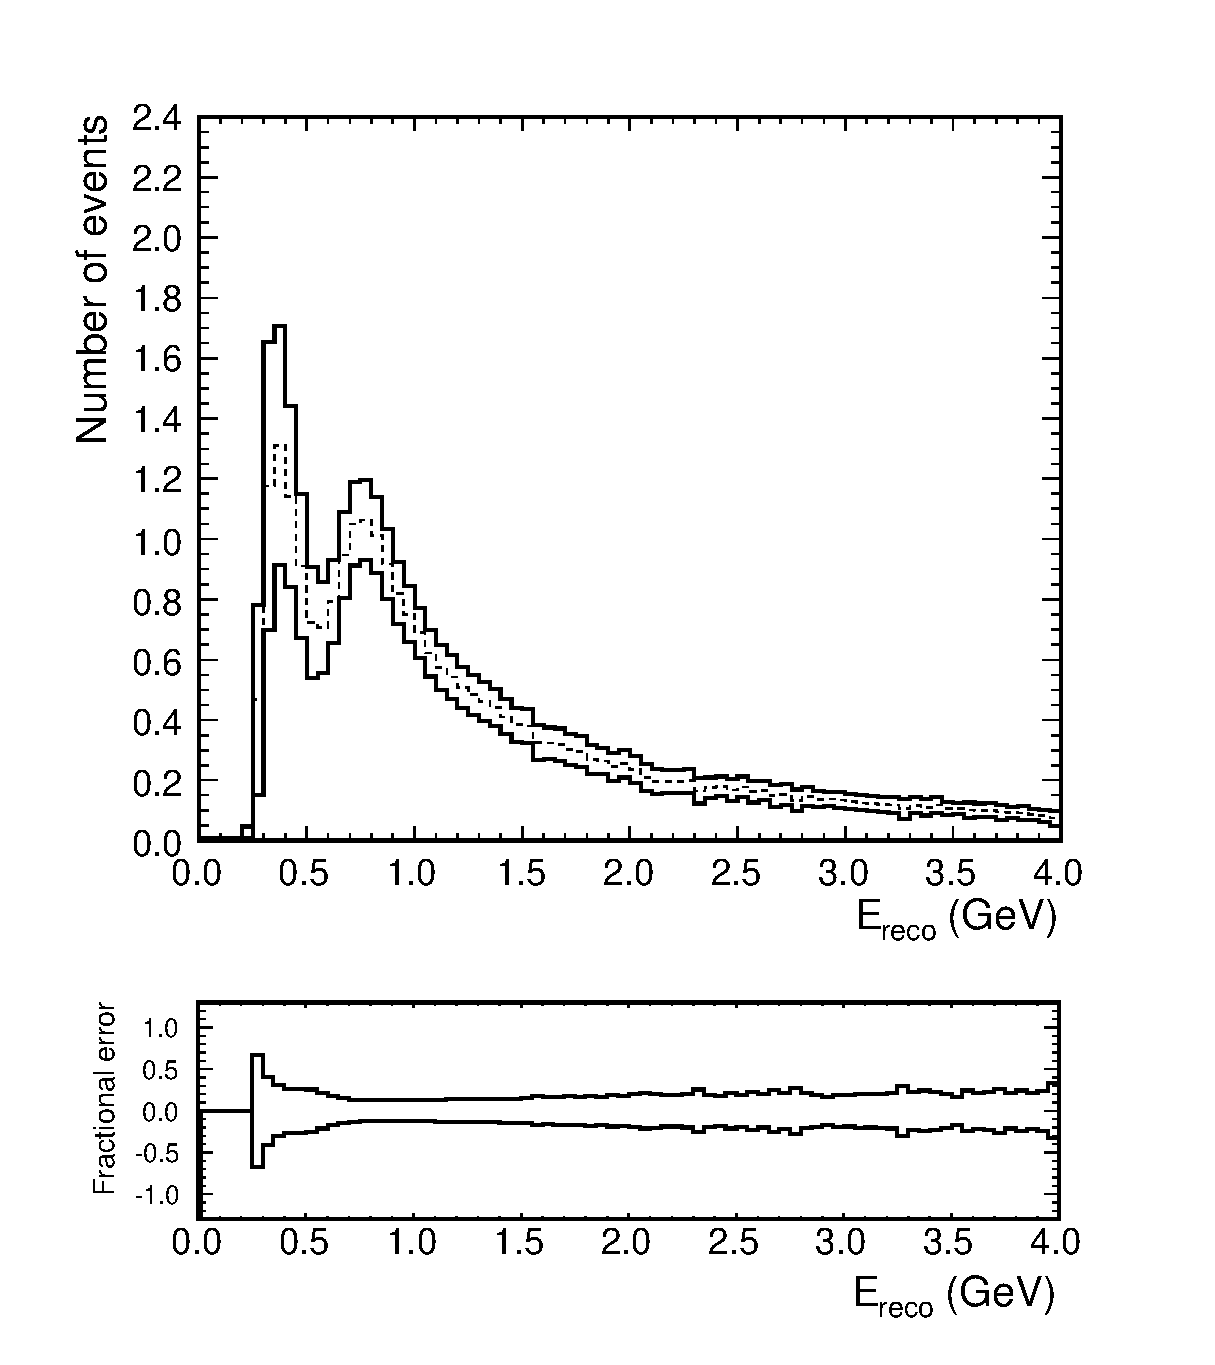
\includegraphics[width=18pc,height=20pc]{images/predicted_spectrum/systematic_variations/neut-sk-err-envelope-minos11.eps}
\caption{
  Error envelope of 1 $\mu$-like ring event reconstructed-energy spectrum (after extrapolation)
  for oscillations with $sin^{2}2\theta_{23}$ = 1.0 and $|\Delta m^{2}_{23}|$ = 2.32$\times10^{-3}$ $eV^{2}/c^{4}$.
  Calculated from toy MC experiments as the $\pm1\sigma$ spread of bin contents (NEUT).
}
\label{fig:neut-sk-err-envelope-minos11}
\end{minipage}
\end{figure}
